\section{Scatterplot characterization}
\label{sec:visualizer:scatterplot}

\subsection{Characteristics of a ``good'' plot}
\label{sec:visualizer:scatterplot:goodplot}

The simplest scatterplot is the response against the observed variables. This,
however, may not be the best way to ascertain independence for the user. This
notion is illustrated in Figure~\ref{fig:visualizer:cdf}. The left plot appears
to be independent as it's a cluster of points near the origin, but it's not
entirely clear due to the multitude of stray points outside of $y\in (-2,2)$ 
and $x\in(-1.5,1.5)$. By looking at the outliers, it could also be argued that 
there is some dependency. However, applying the CDF in both directions creates 
a plot distributed on (0,1). This transformation is non-destructive and 
preserves dependency in the data if it exists. The data is clearly independent 
as the points appear to be uniformly distributed within the box.

\begin{figure}[htb]
	\begin{center}
		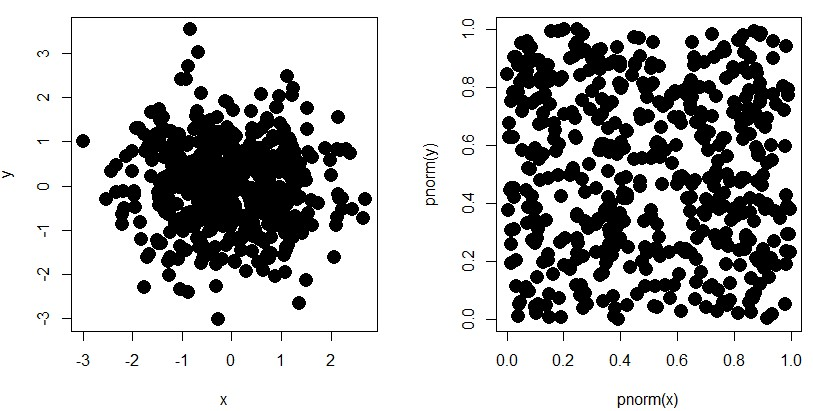
\includegraphics[width=0.75\linewidth]{ch-visualizer/figures/cdf}
		\caption[A plot of $y$ against $x$ after the CDF is applied in both
		directions.]{A plot of $y$ against $x$ with no transformation (left) 
		and after
			the CDF is applied in both directions (right). The code for this 
			example may be
			found in Appendix~\ref{sec:appendicies:cdf}}
		\label{fig:visualizer:cdf}
	\end{center}
\end{figure}

Restricting the plot to a unit box allows analyst's visual systems to focus on
locations where there is low spatial frequency, which is ideal for detecting
dependence~\cite{hofert2016}. The effects of this can be progressively observed
by looking from the left to the right in
Figure~\ref{fig:visualizer:hofertoldford} below.

\begin{figure}[htb]
	\begin{center}
		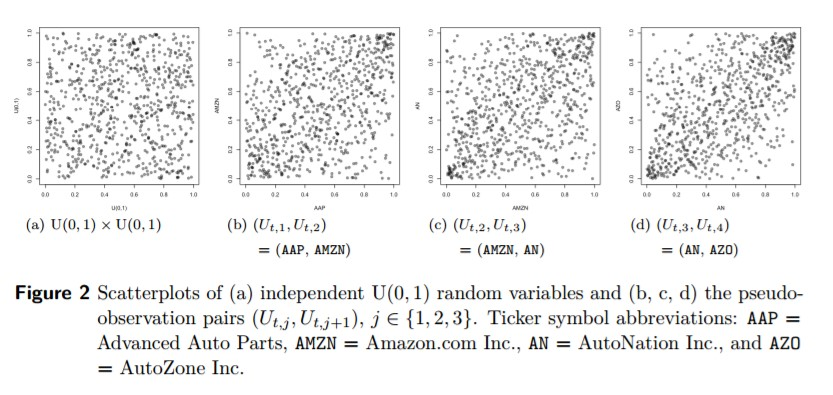
\includegraphics[width=1\linewidth]{ch-visualizer/figures/hofertoldford}
		\caption[Scatterplots of independent $U(0,1)$ random variables and the
		pseudo-observation pairs $(U_{t,j},U_{t,j+1}),j\in 
		\{1,2,3\}$.]{Scatterplots of
			(a) independent $U(0,1)$ random variables and (b,c,d) the 
			pseudo-observation
			pairs $(U_{t,j},U_{t,j+1}),j\in \{1,2,3\}$. Ticker abbreviations: 
			AAP = Advanced
			Auto Parts, AMZN = Amazon.com Inc, AN = AutoNation Inc., AZO = 
			AutoZone Inc.
			Figure from Hofert and Oldford 2016~\cite{hofert2016}}
		\label{fig:visualizer:hofertoldford}
	\end{center}
\end{figure}

\subsection{Feature extraction from plot}
\label{sec:visualizer:scatterplot:features}

In order for the active learning classifier to properly understand and classify 
all $d \choose 2$ plots 
(Sections~\ref{sec:visualizer:al}~\ref{sec:visualizer:plotgeneration}), the 
features must be extracted from each plot. The more useful criteria there are, 
the more sophisticated the classification will be.

\subsubsection{Numerical features}

Our goal is to quantify various features of a scatter plot for the computer, 
and that does include numerical features. The following features are currently 
implemented in the VS: 

\tablespacing
\begin{itemize}
	\item Correlation coefficients and their $p$-values (See 
	Section~\ref{sec:intro:correlation} for more details on the various types 
	of quantifiers)
	\item Kullback-Leibler divergence criterion
	\item Chi-square test of independence and its $p$-value
\end{itemize}
\bodyspacing 

\subsubsection{Visual features}

What is more challenging is to find a way to quantify the visual features of 
scatter plots. This may be done by looking for concentration of points in 
various spaces of the plot domain. The following features are currently 
implemented in the VS: 

\tablespacing
\begin{itemize}
	\item Middle box criterion: Percentage of points near the center of the plot
	\item LR criterion: The percentage of points that lie above and below the 
	linear regression line
	\item Clustering criterion: The percentage quantile of the ratio between 
	the largest and next-largest distance
	\item Visual trend criterion: A higher value suggests a greater visual 
	trend. This is computed by max(PosTrendCriterion, NegTrendCriterion) which 
	is computed from the percentage of points in the upper left and bottom 
	right, and bottome left and upper right, respectively
\end{itemize}
\bodyspacing